\documentclass[UTF8]{ctexart}
\usepackage[a4paper, top = 3cm, bottom = 3cm, left = 2cm, right = 2cm]{geometry}
\usepackage{graphicx}
\usepackage{fancyhdr}
\pagestyle{plain} % 使用plain样式，页码在页脚居中
\usepackage{amsmath}
\usepackage{float}
\usepackage{caption}
\captionsetup[figure]{labelformat = empty}

\newcommand{\rs}{\text{ rad/s}}
\newcommand{\wc}{\omega_\text{c}}

\begin{document}

\section*{2024-2025学年秋学期《控制工程基础》回忆卷改写}

\begin{center}
    折一只纸鹭
\end{center}

\subsection*{第一题}

已知某机械系统如下图所示，$k_1,k_2$ 为弹簧的刚度系数，$\mu$ 为阻尼器的阻尼系数.

\begin{enumerate}
    \item[(1)] 列出系统的运动微分方程.
    \item[(2)] 画出系统的方块图.
    \item[(3)] 求传递函数 $\dfrac{Y_1(s)}{F_\text{i}(s)}$.
\end{enumerate}

\begin{figure}[H]
    \centering
    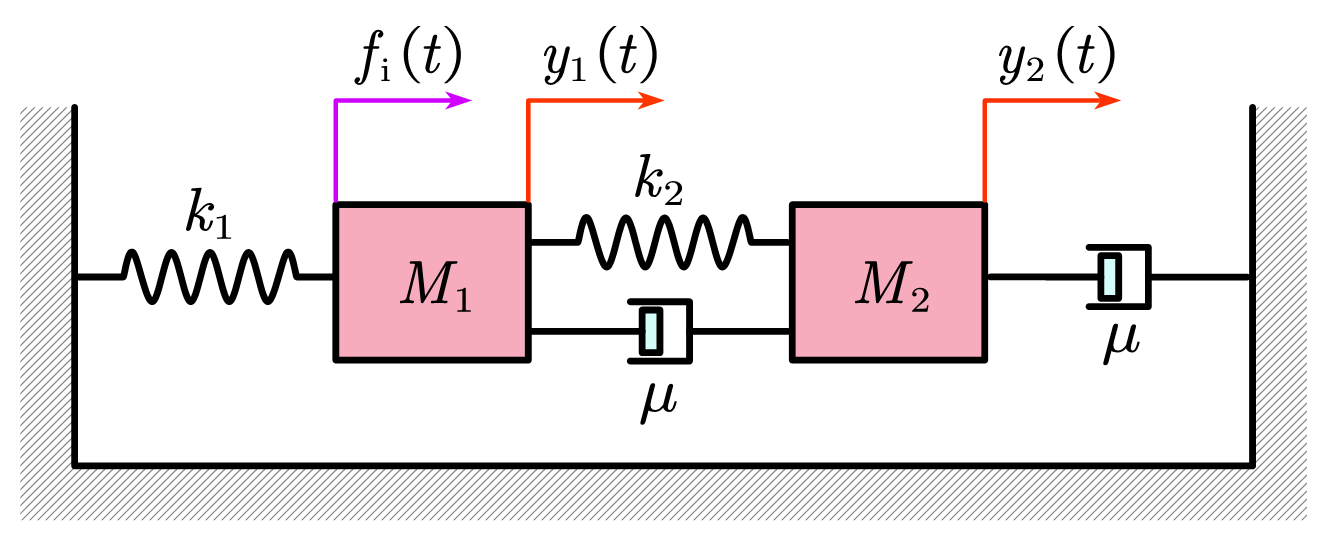
\includegraphics[width=0.6\linewidth]{T1.png}
    \caption{第一题图}
    \label{fig:T1}
\end{figure}

\subsection*{第二题}

给下左图所示的系统施加 330 N 的阶跃力后，$x_\text{o}(t)$ 的时间响应曲线如下右图所示.

\begin{enumerate}
    \item[(1)] 求该系统的质量 $M$、弹性刚度 $k$、黏性阻尼系数 $D$.
    \item[(2)] 求 $x_\text{o}(t)$ 响应的上升时间 $t_\text{r}$ 与调整时间 $t_\text{s}$.
\end{enumerate}

\begin{figure}[H]
    \centering
    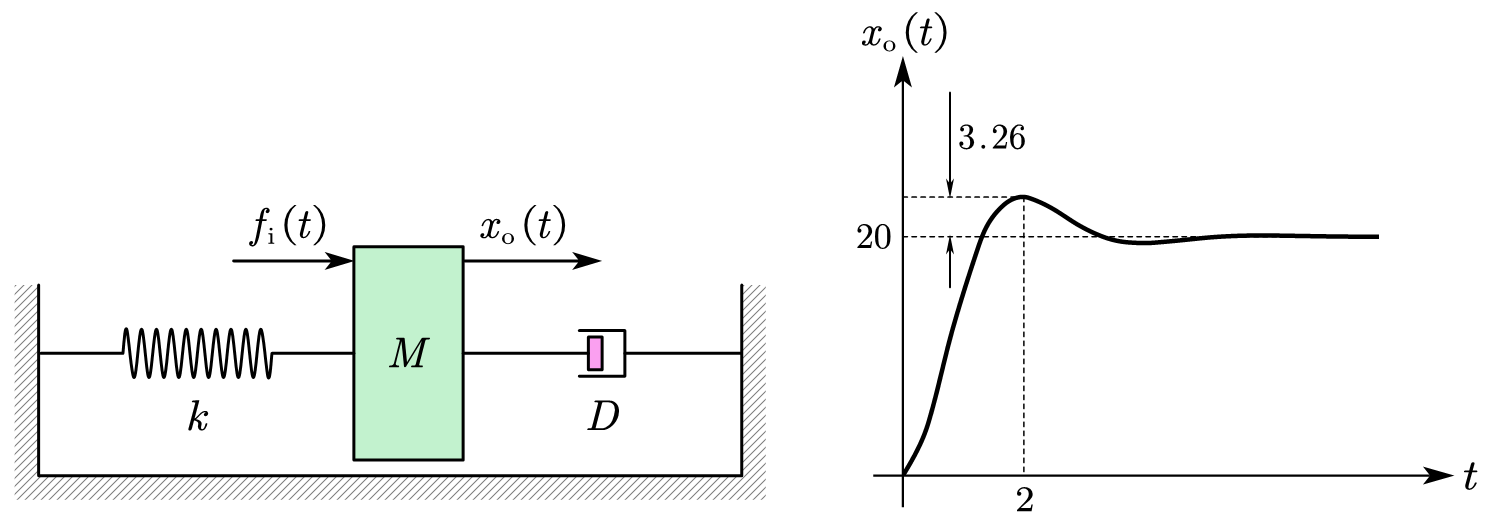
\includegraphics[width=0.8\linewidth]{T2.png}
    \caption{第二题图}
    \label{fig:T2}
\end{figure}

\subsection*{第三题}

某最小相位系统的开环传递函数的幅频图如下所示.

\begin{enumerate}
    \item[(1)] 写出该开环传递函数的表达式.
    \item[(2)] 求该系统的相位裕量 $\gamma$.
    \item[(3)] 若频域放大十倍，则系统性能会如何变化？
    
\end{enumerate}

\begin{figure}[H]
    \centering
    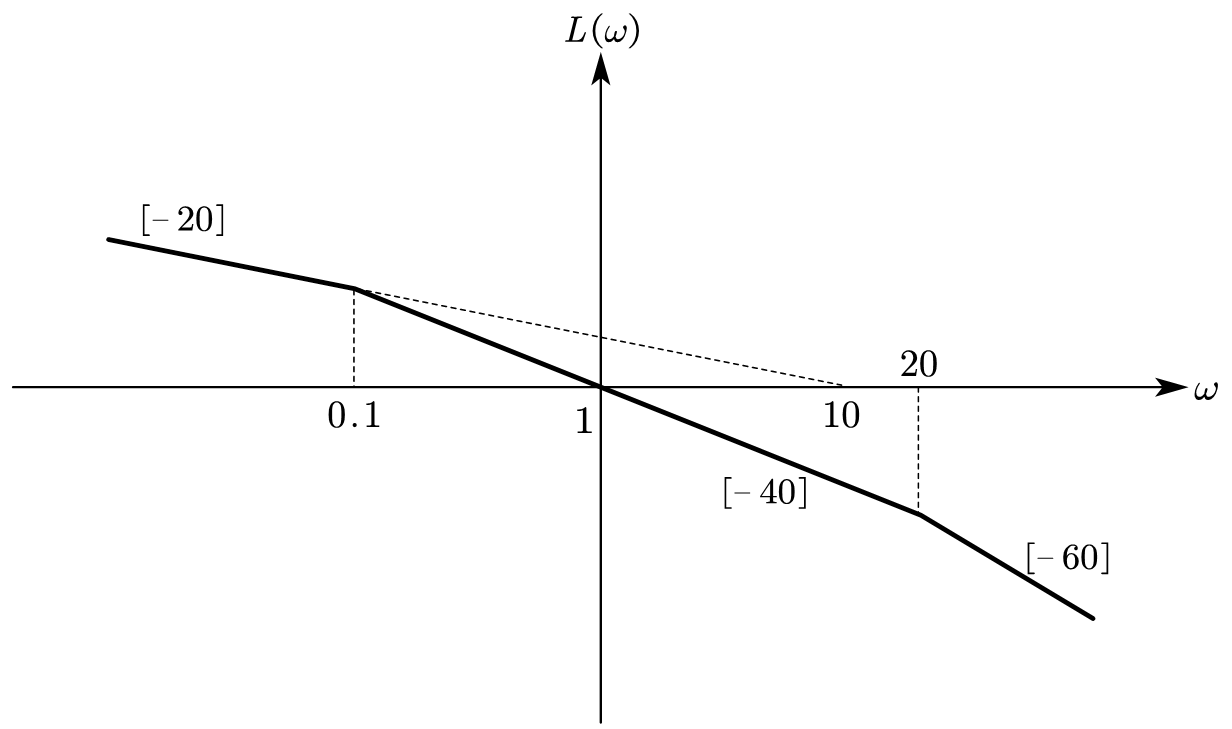
\includegraphics[width=0.75\linewidth]{T3.png}
    \caption{第三题图}
    \label{fig:T3}
\end{figure}

\subsection*{第四题}

设单位反馈系统的开环传递函数
\[
    G(s)=\frac{K}{s(s+2)(s+3)}
\]
用 Nyquist 判据求系统稳定时 $K$ 的取值范围.

\newpage
\subsection*{第五题}

已知系统的方块图如下所示.

\begin{enumerate}
    \item[(1)] 用 Routh 判据求系统稳定时 $K$ 的取值范围.
    \item[(2)] 取 $K=2$，若输入信号 $x_\text{i}(t)=1(t)$，干扰信号 $n(t)=\dfrac{1}{2}\cdot 1(t)$，求系统的稳态误差.
\end{enumerate}

\begin{figure}[H]
    \centering
    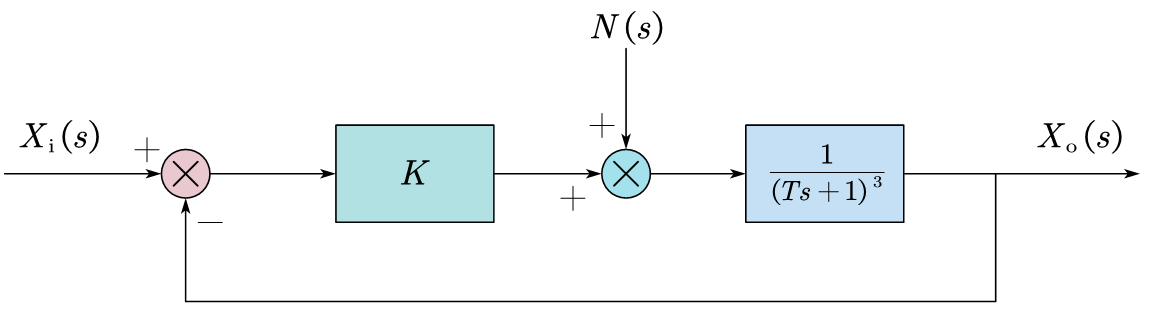
\includegraphics[width=0.75\linewidth]{T5.png}
    \caption{第五题图}
    \label{fig:T5}
\end{figure}

\subsection*{第六题}

已知某单位反馈系统的开环传递函数
\[
G_0(s)=\frac{5}{s(0.1s+1)(0.5s+1)}
\]

\begin{enumerate}
    \item[(1)] 加入一个串联校正环节，使相角裕量 $\gamma\ge 45^\circ$，用超前校正实现.
    \item[(2)] 画出校正前和校正后的幅值 Bode 图.
\end{enumerate}

\subsection*{第七题}

已知某单位反馈系统的开环传递函数
\[
G(s)=\frac{K^*}{s(s+2)(s+5)}
\]

\begin{enumerate}
    \item[(1)] 作 $K^*$ 从 $0\rightarrow\infty$ 时的闭环根轨迹图（请写出详细过程）.
    \item[(2)] 求当 $\xi=0.5$ 时闭环的一对主导极点，并求其 $K^*$ 的值.
\end{enumerate}

\newpage
\section*{2023-2024学年秋学期《控制工程基础》回忆卷改写}

\begin{center}
    折一只纸鹭
\end{center}

\subsection*{第一题（仅考点）}

类似课本习题2-19，需要写出微分方程、方块图和传递函数。

\subsection*{第二题（仅考点）}

给一个单位反馈系统的开环传递函数，求上升时间、峰值时间、调整时间和最大超调量；第二问要求画出二阶震荡系统的时域图然后在图上标出上述量。

\subsection*{第三题}

已知单位反馈系统的开环传递函数为
\[
G(s)=\frac{1000(Ts+1)}{s(s+1)(s+10)}
\]
其中 $0<T<0.1$.

\begin{enumerate}
    \item[(1)] 求系统的开环增益与转折频率.
    \item[(2)] 画出该开环传递函数的幅频图.
    \item[(3)] 要使系统闭环稳定，求 $T$ 的取值范围.
\end{enumerate}

\subsection*{第四题}

已知单位反馈系统的开环传递函数为
\[
G(s)=\frac{-1}{s^2+As+B}
\]
其中 $A,B>0$. 请画出该开环传递函数的 Nyquist 图，并判断系统的闭环稳定性.

\subsection*{第五题（仅考点）}

给一个方块图，有输入和扰动，第一问用劳斯阵列判断闭环稳定性，第二问输入单位斜坡，扰动单位阶跃，求稳态误差。\textbf{注意这里不是单位负反馈，有一个反馈函数 $H(s)$。}

\subsection*{第六题}

已知某单位反馈系统的开环传递函数
\[
G_0(s)=\frac{8}{s(0.1s+1)(0.5s+1)}
\]
试加入一个串联校正环节，使相角裕量 $\gamma\ge 35^\circ$.

\begin{enumerate}
    \item[(1)] 若要使剪切频率 $\omega_\text{c}\ge 5 \rs$，请用超前校正实现.
    \item[(2)] 若要使剪切频率 $\omega_\text{c}\le 1.5 \rs$，请用滞后校正实现.
\end{enumerate}

\newpage
\section*{2022-2023学年秋学期《控制工程基础》回忆卷改写}

\begin{center}
    折一只纸鹭
\end{center}

\subsection*{第一题（仅考点）}

给一个一维阻尼系统，求运动方程，画方块图，写传递函数。

\subsection*{第二题（仅考点）}

给一个二阶振荡模型与时域特性曲线，给超调量、上升时间、时域稳定值，求二阶震荡的系数（用超调量、上升时间、终值定理列方程组）。

\subsection*{第三题（仅考点）}

给一个简单的传递函数，画 Bode 图，求剪切频率与相位裕量。

\subsection*{第四题（原帖第五题）}

某单位反馈系统的开环传递函数为
\[
G(s)=\frac{K(s+2)}{s(s-2)}
\]
其中 $K>0$. 请画出该开环传递函数的 Nyquist 图，并判断系统的闭环稳定性.

\subsection*{第五题（仅考点，原帖第四题）}

给一个方块图，图里有输入与干扰，先判稳定性（代数判据），再求稳态误差（两个相加）。

\subsection*{第六题}

某单位反馈系统的固有部分的传递函数为
\[
G_0(s)=\frac{K}{s(0.008s+1)(0.002s+1)(0.001s+1)}
\]

\begin{enumerate}
    \item[(1)] 若要使速度误差系数 $K_\text{v}=200\rs$，剪切频率 $\wc\le 30 \rs$，相位裕度 $\gamma\ge50^\circ$，试确定 $K$ 的值，并设计串联滞后校正.
    \item[(2)] 画出校正前和校正后的幅值 Bode 图.
    \item[(3)] 利用高阶最优模型，优化系统中的小时间常数环节（0.008、0.002、0.001）.
\end{enumerate}

\subsection*{第七题}

某单位反馈系统的开环传递函数为
\[
G(s)=\frac{s(s+1)}{s+a}
\]
画出以 $a$ 为参量的根轨迹图（$a$ 从 $0\rightarrow\infty$）.

\end{document}
